\chapter{List of Components}
\label{app:components}
\begin{table}[h]
    \centering
    \begin{tabular}{lllll}
        Retailer    & Amount & Price NOK/unit & Part Number            & Name                        \\
        \hline
        Digikey     & 3      & 8,66          & ADP170AUJZ & Voltage regulator           \\
        Farnell     & 3      & 121,35        & 1210018                & SARONIX  CRYSTAL OSCILLATOR \\
        Farnell     & 20     & 1,5           & 2251493                & LEDS                        \\
        Farnell     & 10     & 19,5          & 2356206                & Header pins                 \\
        Farnell     & 100    & 0.0118        & 2367994                & FPC-HEADER                  \\
        Farnell     & 20     & 5.1           & 1593446                & Header pins                 \\
        Farnell     & 4      & 105,75        & 2103743                & AS7C38098A                  \\
        Farnell     & 2      & 601,95        & 1876230                & FPGA                        \\
        Farnell     & 2      & 85,52         & 2314200                & EFM                         \\
        Farnell     & 20     & 2,45          & 1217764                & Button                      \\
        Farnell     & 6      & 6,15          & 9778195                & LM1117MP-3.3                \\
        Farnell     & 10     & 14,40         & 1654540                & HDMI                        \\
        Farnell     & 6      & 22,0          & 1842014                & EFM crystal                 \\
        Farnell     & 2      & 157,86        & 2302279                & RPi camera                  \\
        Farnell     & 30     & 1             & 1653253                & 10k$\Omega$ resistor            \\
        Farnell     & 30     & 0             & 1469803                & 330$\Omega$ resistor            \\
        Farnell     & 30     & 0             & 2309108                & 1k$\Omega$ resistor             \\
        Farnell     & 30     & 0             & 2112878                & 50$\Omega$ resistor             \\
        Farnell     & 30     & 0             & 1652884                & 4.7k$\Omega$ resistor           \\
        Farnell     & 30     & 0.126         & 2333587                & 100$\Omega$ resistor            \\
        Farnell     & 20     & 2,09          & 2211173                & 4.7$\mu$F capacitor             \\
        Farnell     & 20     & 1.55          & 2346908                & 0.47$\mu$F capacitor            \\
        Farnell     & 40     & 0             & 9406140                & 0.1$\mu$F capacitor             \\
        Farnell     & 20     & 2,35          & 2309028                & 10$\mu$F capacitor              \\
        Farnell     & 20     & 1.49          & 2211179                & 1$\mu$F capacitor               \\
        Farnell     & 20     & 13,82         & 2494476                & 100$\mu$F capacitor
    \end{tabular}
    \caption{List of components}
    \label{listofcomponents}
\end{table}

\chapter{Pinouts}
\label{app:pinouts}
\begin{table}[h]
    \centering
    \begin{tabular}{lllll}
        HDMI Pin Name            & Header Pin Nr & FPGA HDMI 1 & FPGA HDMI 2 & External \\
        \hline
        TMDS Data2+              & 3             & B2              & B9              &          \\
        TMDS Data2-              & 5             & A2              & A9              &          \\
        TMDS Data1+              & 7             & D6              & D11             &          \\
        TMDS Data1-              & 9             & C6              & C11             &          \\
        TMDS Data0+              & 10            & B3              & C10             &          \\
        TMDS Data0-              & 8             & A3              & A10             &          \\
        TMDS Clock+              & 6             & B4              & G9              &          \\
        TMDS Clock-              & 4             & A4              & F9              &          \\
        CEC                      & N/C           & N/C             &                 &          \\
        HEC Data (Opt)           & GND           & N/C             &                 &          \\
        SCL                      & N/C           & N/C             &                 &          \\
        SDA                      & N/C           & N/C             &                 &          \\
        DDC                      & GND           & N/C             &                 &          \\
        5+ Power                 & P15 Header    & N/C             &                 &          \\
        Hot Plug Detect          & N/C           & N/C             &                 &          \\
        HP Detect (HDMI1) & P9 Header     & N/C             &                 &          \\
        GND & 1             &                 &                 & GND      \\
        VCC & 2             &                 &                 & VCC      \\
    \end{tabular}
    \caption{HDMI Connector}
    \label{HDMI_Connector}
\end{table}

\begin{figure}
    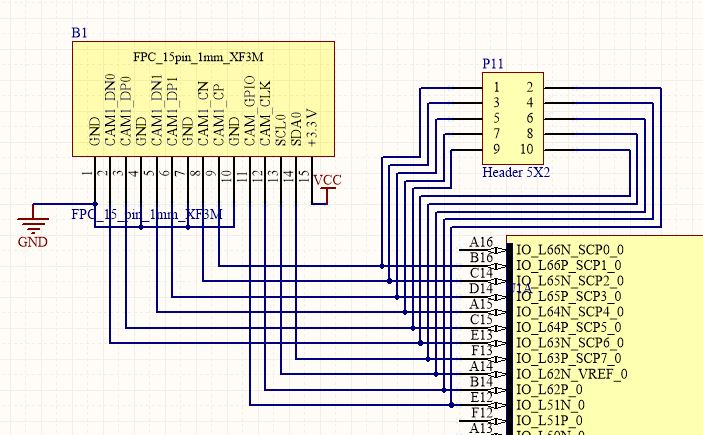
\includegraphics[width=\linewidth]{img/fpc_header.jpg}
    \caption{Raspberry Pi connector}
    \label{fig:FpcHeader}
\end{figure}

% Is the column with pull-up really necessary?
\begin{table}[]
    \centering
    \begin{tabular}{llll}
        Button & Connection & Pull-up/pull-down & Name     \\
        \hline
        SW6    & FPGA P15   & Pull-up          &          \\
        SW7    & FPGA P16   & Pull-up          &          \\
        SW1    & EFM PD8    & Pull-up          & BTN OK   \\
        SW2    & EFM PD7    & Pull-up          & BTN Back \\
        SW3    & EFM PD6    & Pull-up          & BTN Down \\
        SW4    & EFM PD5    & Pull-up          & BTN Up   \\
        SW5    & EFM K6     & Pull-up          & Reset
    \end{tabular}
    \caption{I/O buttons}
    \label{tab:Buttons}
\end{table}

\begin{table}[]
    \centering
    \begin{tabular}{llll}
        Pin number & EFM pin & Usage & Shared with \\
        \hline
        1       & PB4     & I/O   &             \\
        2       & PA7     & I/O   &             \\
        3       & PB5     & I/O   &             \\
        4       & PA8     & I/O   &             \\
        5       & PB6     & I/O   &             \\
        6       & PA9     & I/O   &             \\
        7       & PB7     & I/O   &             \\
        8       & PA10    & I/O   &             \\
        9       & PB8     & I/O   & INIT\_B     \\
        10      & PA11    & I/O   &             \\
        11      & PB11    & I/O   & Program\_B  \\
        12      & PC0     & I/O   &             \\
        13      & PB12    & I/O   & Done        \\
        14      & PC1     & I/O   &             \\
        15      & PB15    & I/O   &             \\
        16      & PC9     & I/O   &             \\
        17      & PD4     & I/O   &             \\
        18      & PC10    & I/O   &             \\
        19      & PD11    & I/O   &             \\
        20      & PC11    & I/O   &             \\
        21      & PD12    & I/O   &             \\
        22      & PF11    & I/O   &             \\
        23      & PD13    & I/O   &             \\
        24      & PF10    & I/O   &             \\
        25      & PF5     & I/O   &             \\
        26      & PF7     & I/O   &             \\
        27      & PF6     & I/O   &             \\
        28      & 3.3V    &       &
    \end{tabular}
    \caption{Header outputs}
    \label{tab:HeaderOut}
\end{table}

\begin{figure}
    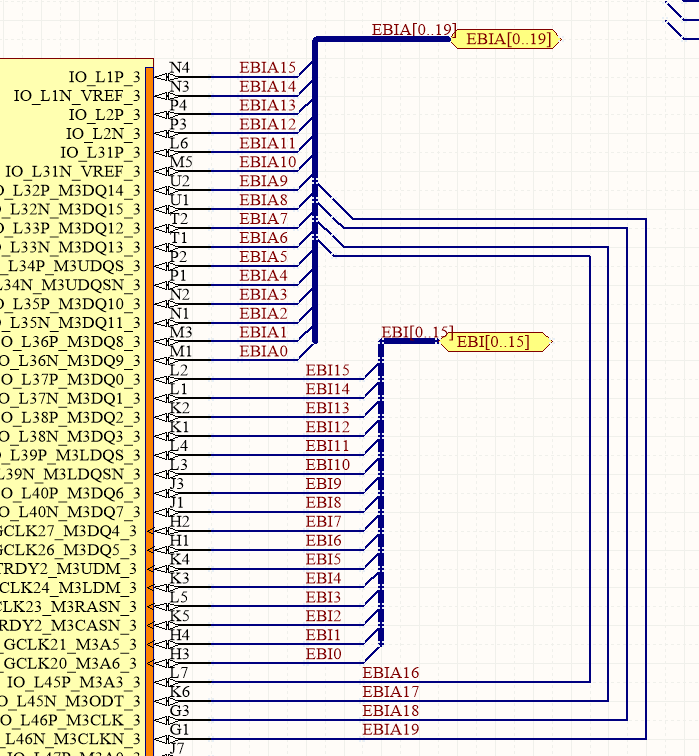
\includegraphics[width=\linewidth]{img/EBI-bus.png}
    \caption{EBI bus input}
    \label{fig:EbiBus}
\end{figure}

\begin{figure}
    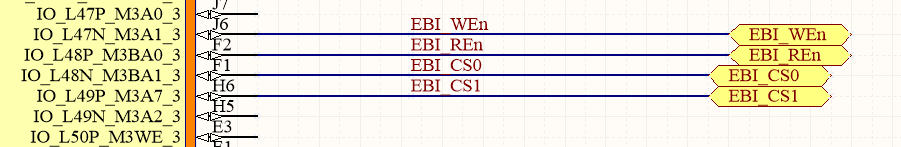
\includegraphics[width=\linewidth]{img/EBI-bus_2.png}
    \caption{EBI bus control signals}
    \label{fig:EbiControl}
\end{figure}

\chapter{PCB Schematics}

\begin{figure}
    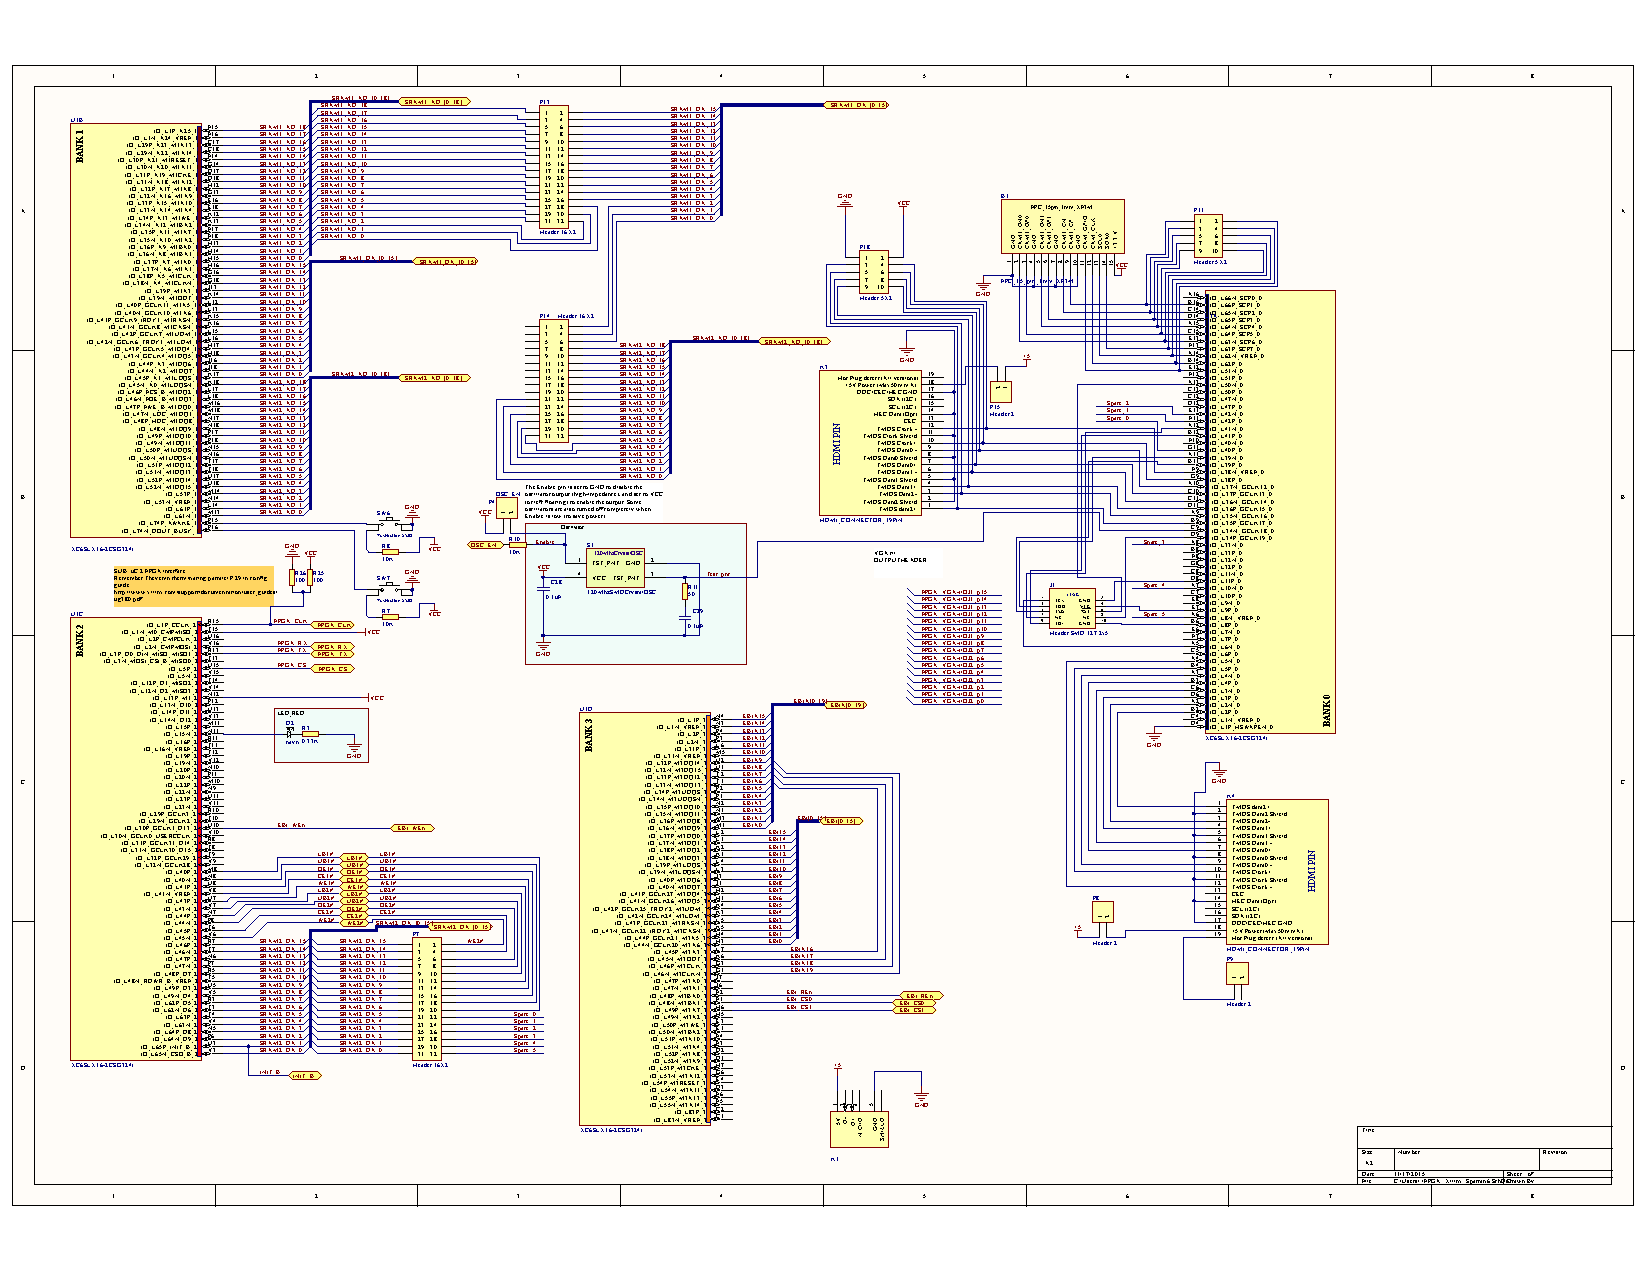
\includegraphics[width=\linewidth]{img/FPGA_Xilinx_Spartan6.pdf}
    \caption{Xilinx Spartan-6 FPGA}
    \label{fig:FPGA_Xilinx_Spartan6}
\end{figure}

\begin{figure}
    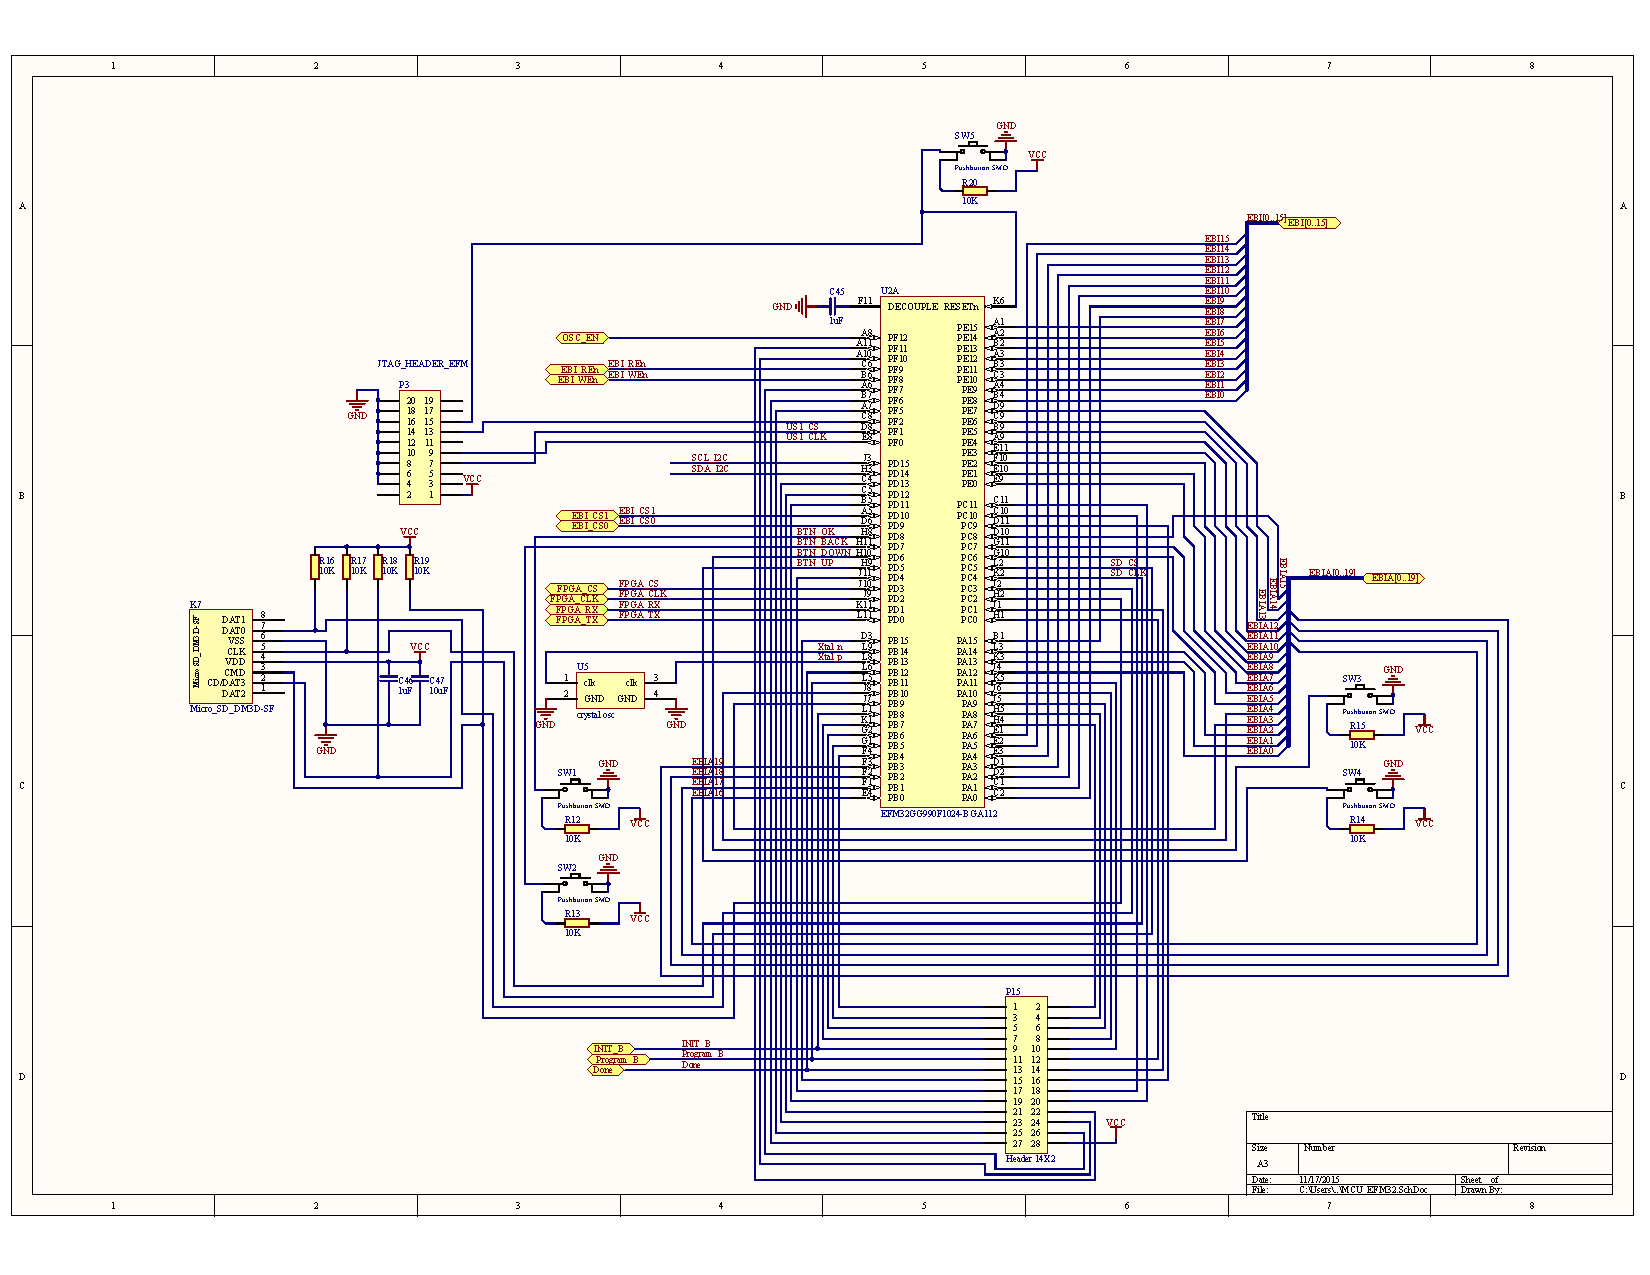
\includegraphics[width=\linewidth]{img/MCU_EFM32.pdf}
    \caption{Silicon Labs EFM32 MCU}
    \label{fig:MCU_EFM32}
\end{figure}

\begin{figure}
    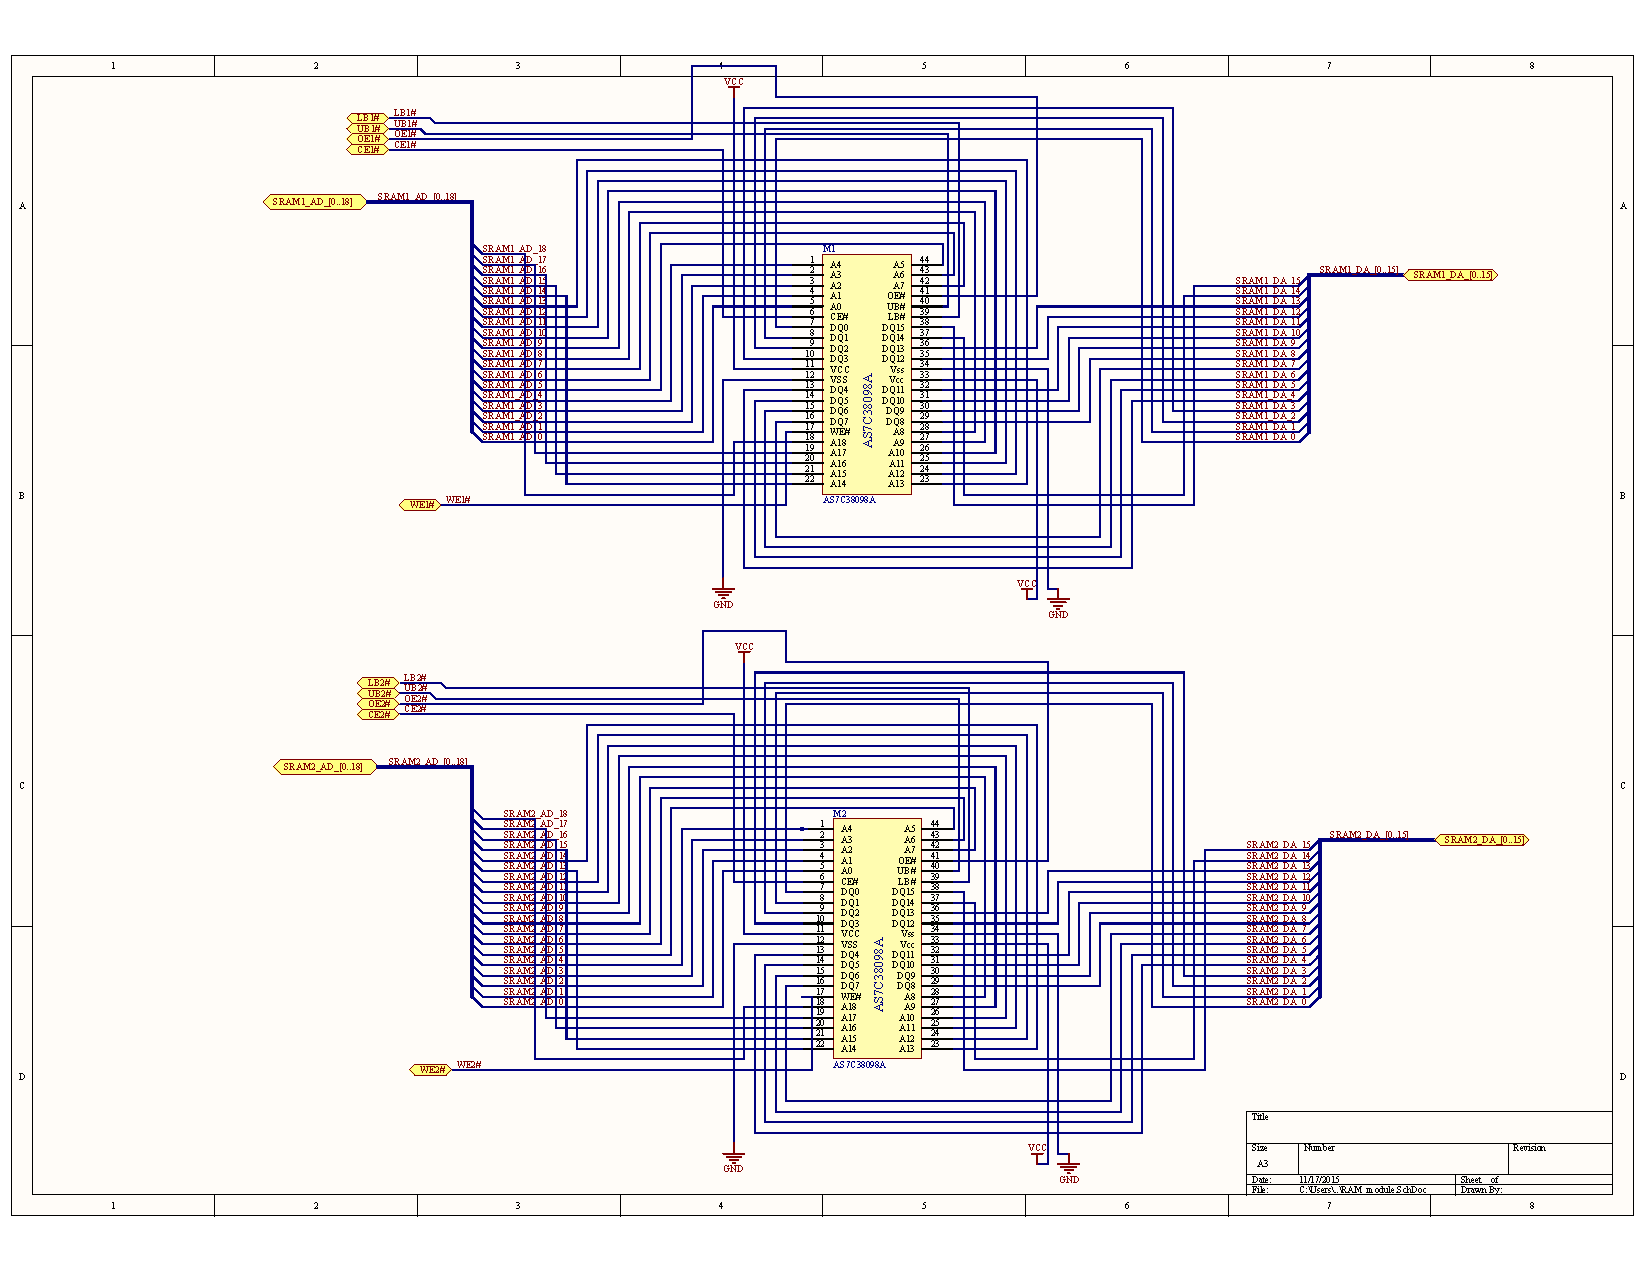
\includegraphics[width=\linewidth]{img/RAM_module.pdf}
    \caption{SRAM module}
    \label{fig:RAM_module}
\end{figure}

\begin{figure}
    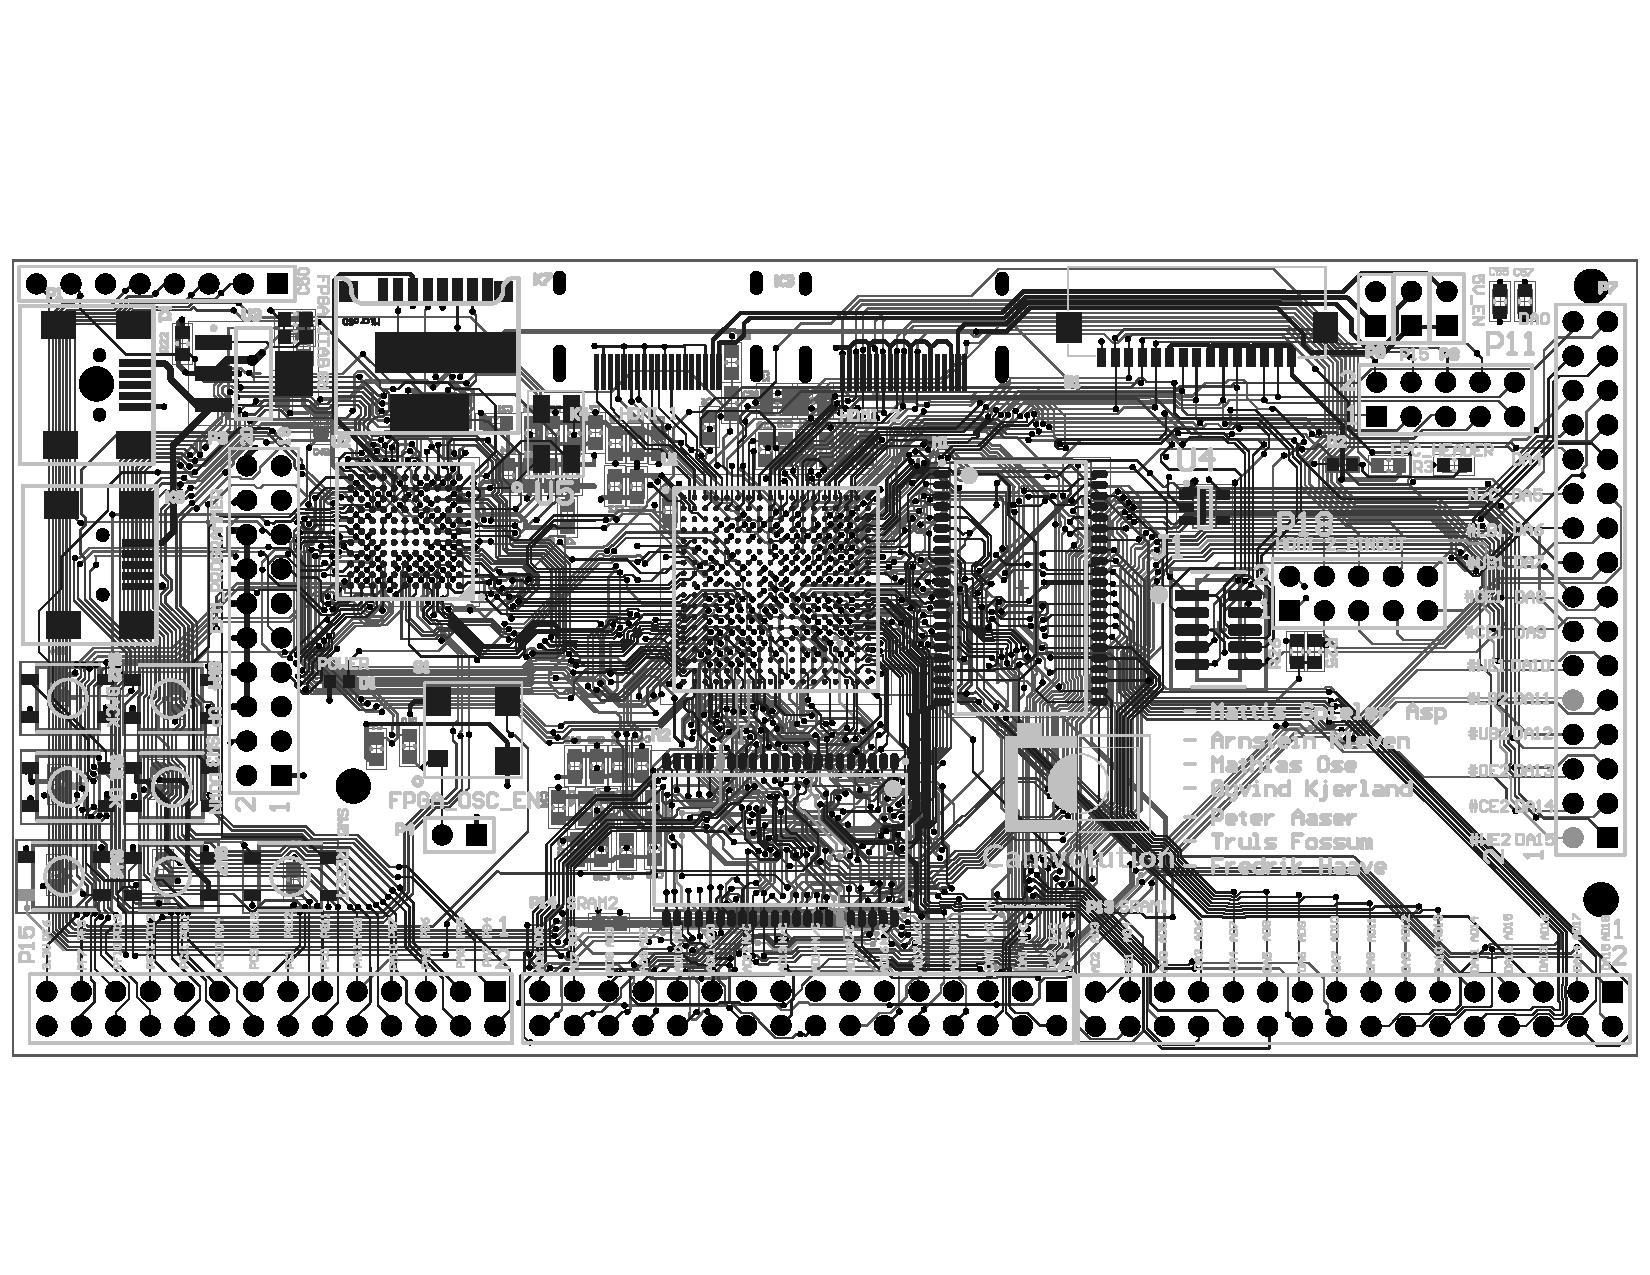
\includegraphics[width=\linewidth]{img/PCB_Finished.pdf}
    \caption{Finished PCB}
    \label{fig:PCB_Finished}
\end{figure}

\chapter{Assignment Text}
\label{app:assignment_text}
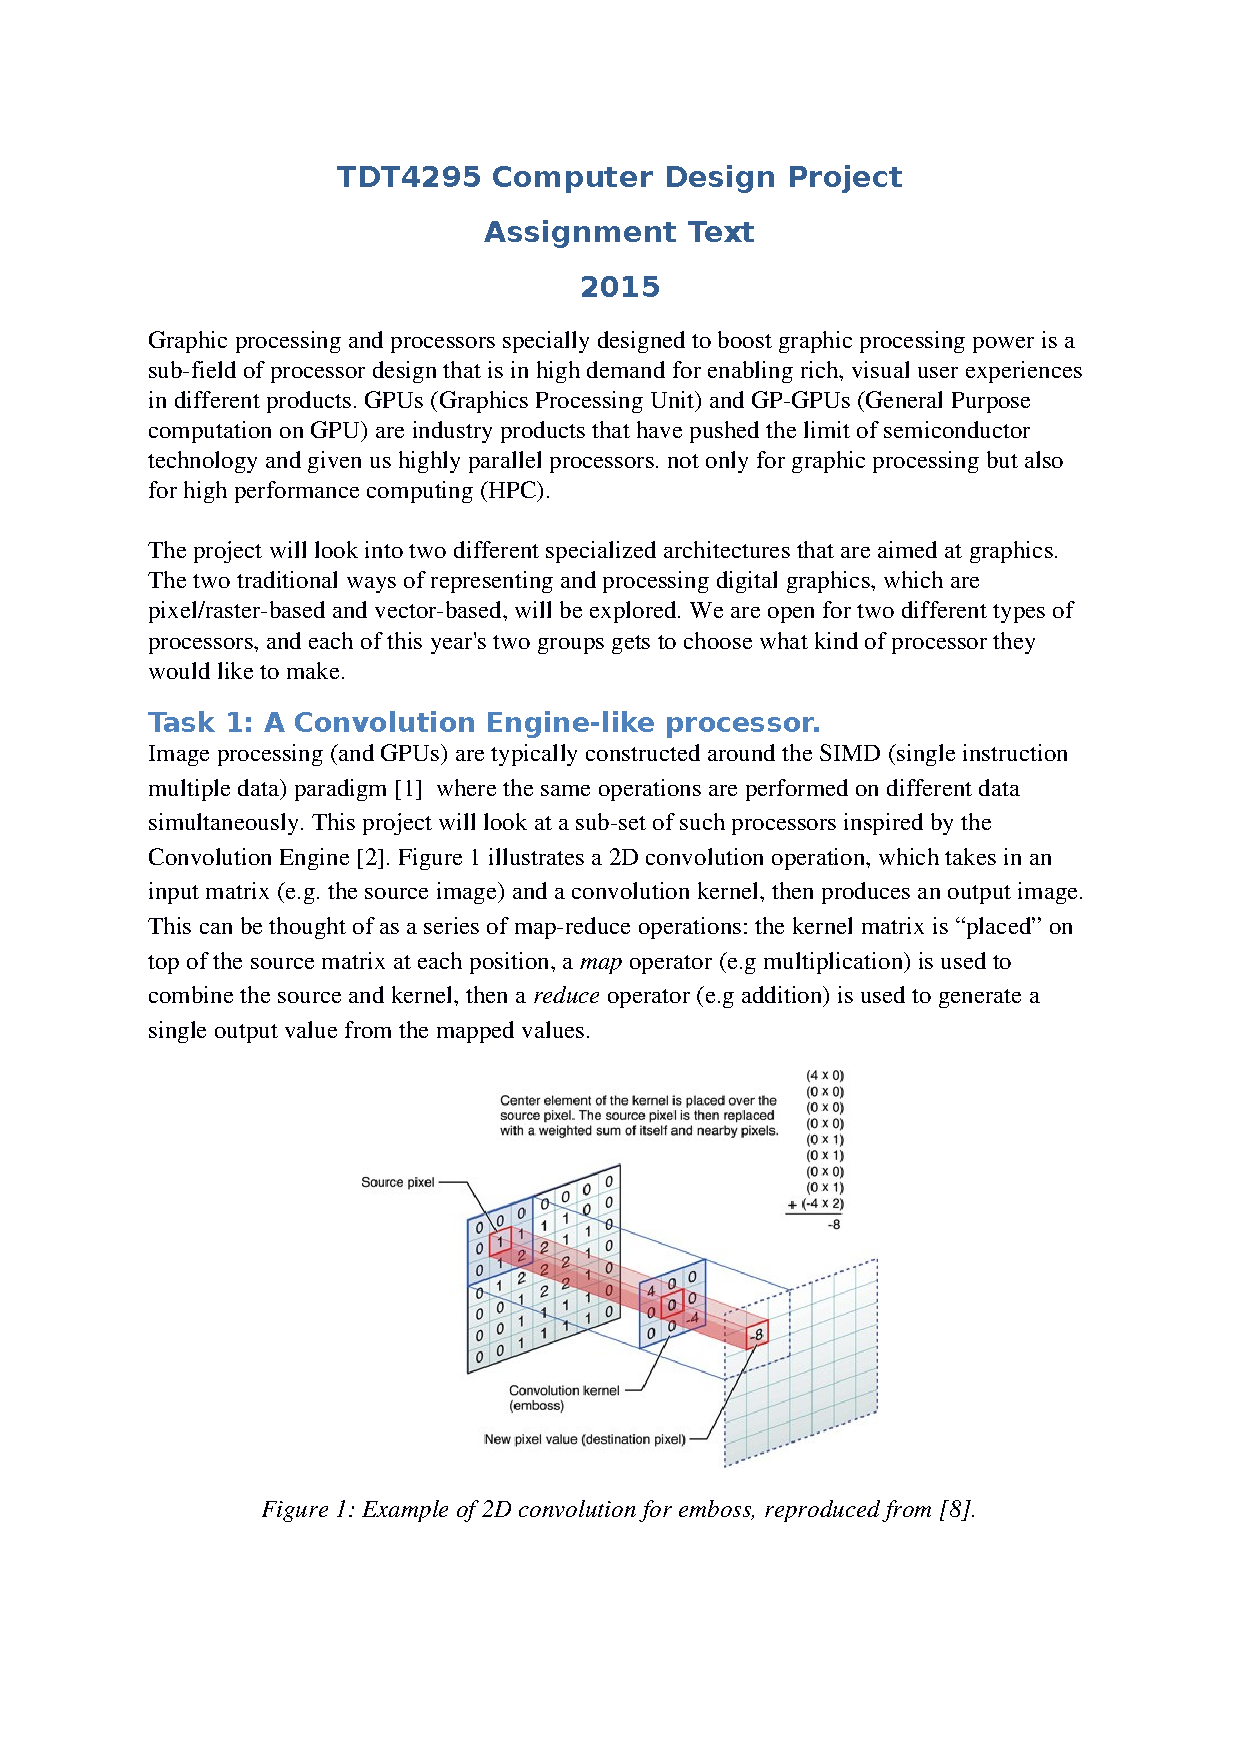
\includepdf[pages={1-},scale=1.0]{img/assignment-text-2015.pdf}


